\chapter{EXPERIMENTS}
\label{chap:experiments}

In this chapter, we will compare execution times of our algorithm's code(henceforth referred to as \textbf{cuML}) against some of the libraries mentioned in \cref{tab:otherlibs}, namely \textbf{gplearn}, \textbf{KarooGP}(only GPU), and \textbf{TensorGP}(both CPU and GPU). The evaluation time for each library is computed for synthetically generated 2D datasets of sizes ranging from $4096$ to $4$ million datapoints for an average over $10$ runs. 

Before exploring the setup for the experiments, we note that field of GP, especially for Symbolic Regression suffers from a lack of standardized benchmarks. This problem is explored by a few studies \citep{GP_Better_Benchmarks}\citep{Orzechowski_2018}, which attempt to quantify and list candidate GP problems. In our experiments, we try to follow the guidelines laid out in these studies.

Our experiments were motivated by \citep{baeta2021speed}, and follow a similar flow for testing execution times between different libraries. All experiments were carried out in a laptop with the spefications listed in \cref*{tab:laptop}.

\begin{table}[htbp]
  \caption{Hardware and software setup for carrying out all experiments}
  \begin{center}
      \begin{tabular}[c]{cc}%{|>{\bf}c|c|}
        \toprule
        \textbf{Component} &   \textbf{Specification} \\
        \midrule
        CPU & Intel i5-9300H (8) @ 4.100GHz \\
        GPU & Nvidia GeForce GTX 1650       \\
        RAM & 8 GB                          \\
        OS  & Ubuntu 20.04.2 LTS            \\
        GPU-RAM& 4 GB          \\
        \bottomrule
      \end{tabular}
      \label{tab:laptop}
  \end{center}
\end{table}

\section{Setup}
\label{sec:setup}
\subsection{Synthetic Data Generation}
\label{subsec:datagen}
In all symbolic regression runs, we try to approximate the Pagie Polynomial\citep{Pagie1997} over the domain $(x,y) \in [-1,1] \times [-1,1]$.

\begin{align}
  f(x,y) = \frac{1}{1 + x^{-4}} + \frac{1}{1 + y^{-4}}
\end{align}

We generate $6$ synthetic datasets by uniformly subsampling datapoints from the domain $(x,y) \in [-1,1] \times [-1,1]$. The initial dataset is generated by subsampling a random square grid of dimensions $64 \times 64 = 4096$ points from the domain. To generate the remaining datasets, the length of the grid is iteratively doubled until we subsample a grid of side $2048$ containing over $4$ million datapoints.

\subsection{Runtime configurations}
\label{subsec:rtconfig}
We detail the runtime configurations for all libraries being benchmarked below. 
\subsubsection{cuML} 
There are no changes to the core algorithm. Once the dataset is loaded into memory, $10$ training runs of $50$ generations are benchmarked for execution time. In addition, best and average fitness values over the generation history is also recorded after the completion of the first run. Execution time is logged using CUDA Events.\\
Note that there is no need to compute fitness values for all $10$ runs as the training runs are designed to be reproducible. 

\subsubsection{gplearn}
The benchmark approach used for cuML is also adopted for training a gplearn regressor. The only notable difference here is that every gplearn run is parallelized using $\mathbf{8}$ jobs (using the Python joblib library).

\subsubsection{KarooGP}
For the KarooGP library, we modify the provided server script to allow running multiple runs at once. Timings for each run are then logged for all input datasets. We consider only the GPU parallelized TensorFlow variant of this library.   

\subsubsection{TensorGP}
TensorGP already has an example script for computing and benchmarking execution time. This script was modified and the execution time already logged by the internal GP Engine is used for our inferences.

For TensorGP, we consider the execution time for both the CPU and GPU TensorFlow backends in our study.

\subsection{Common Parameters and Comparisons}
\label{subsec:commparams}
% We note that since every library has it's own specific implementation of genetic operators, it is hard exactly reproduce the same behaviour of tree-growth between different libraries. Thus, for all $4$ libraries, we only compute the time taken for execution on our synthetic datasets, with some common training parameters listed in \cref{tab:params}.
 
% However, since cuML's mutation model uses gplearn mutations as a reference, we further analyze 
The common parameters used to run all experiments are detailed in \cref{tab:params}. The Ramped Half and Half method was used for tree initialization in all libraries. In the experiment, other than inserting code to compute execution time across generations, no library specific code pertaining to mutations or tree initialization was altered.

For all libraries, we used Root Mean Square Error(RMSE) on the training dataset as the fitness metric for all population trees. 

The function set $\{+,-,*,\div,\sin ,\cos,\tan\}$ was used for all GP runs 

We then compare the variation of best tree fitness across generations on a train-test split of the synthetic datasets only for cuML and gplearn, since cuML essentialy re-implements gplearn's evolution model, albeit on the GPU. 

Note that this kind of analysis isn't possible for the other libraries, since each library has it's own specific mutation model and random number generator for tree generation. 

\begin{table}[htbp]
  \caption{Common parameters used for comparing execution time across libraries}
  \begin{center}
    \begin{tabular}[c]{cc}
      \toprule
      \textbf{Parameter} & \textbf{Value} \\
      \midrule
      Runs                      & 10      \\
      Number of Generations     & 50      \\
      Population size           & 50      \\
      Tournament size           & 4       \\ 
      Generation Method         & Ramped Half and Half \\
      Fitness Metric            & RMSE    \\
      Crossover probability     & 0.7     \\
      Mutation probability      & 0.25    \\
      Reproduction probability  & 0.05    \\
      Domain range              & [-1,1]  \\
      Function Set              & $\{+,-,*,\div,\sin ,\cos,\tan\}$ \\
      \bottomrule
    \end{tabular}
    \label{tab:params}
  \end{center}
\end{table}

\section{Experimental Results}
\label{sec:results}
A total of $290$ runs were performed across the $5$ different GP libraries to produce the results in this section. We compare the average execution time for $10$ runs on $4096$ to $4$ million datapoints, followed by an analysis of the evolution of fitness for both cuML and gplearn.

\subsection{Execution Time}
\label{subsec:exectimes}
\Cref{fig:exectimes} showcases the variation of execution time with increasing dataset size for different datasets, averaged over $10$ runs on each dataset. The same average values are recorded in \cref{tab:execavgs}

\begin{figure}[htbp]
  \centering
  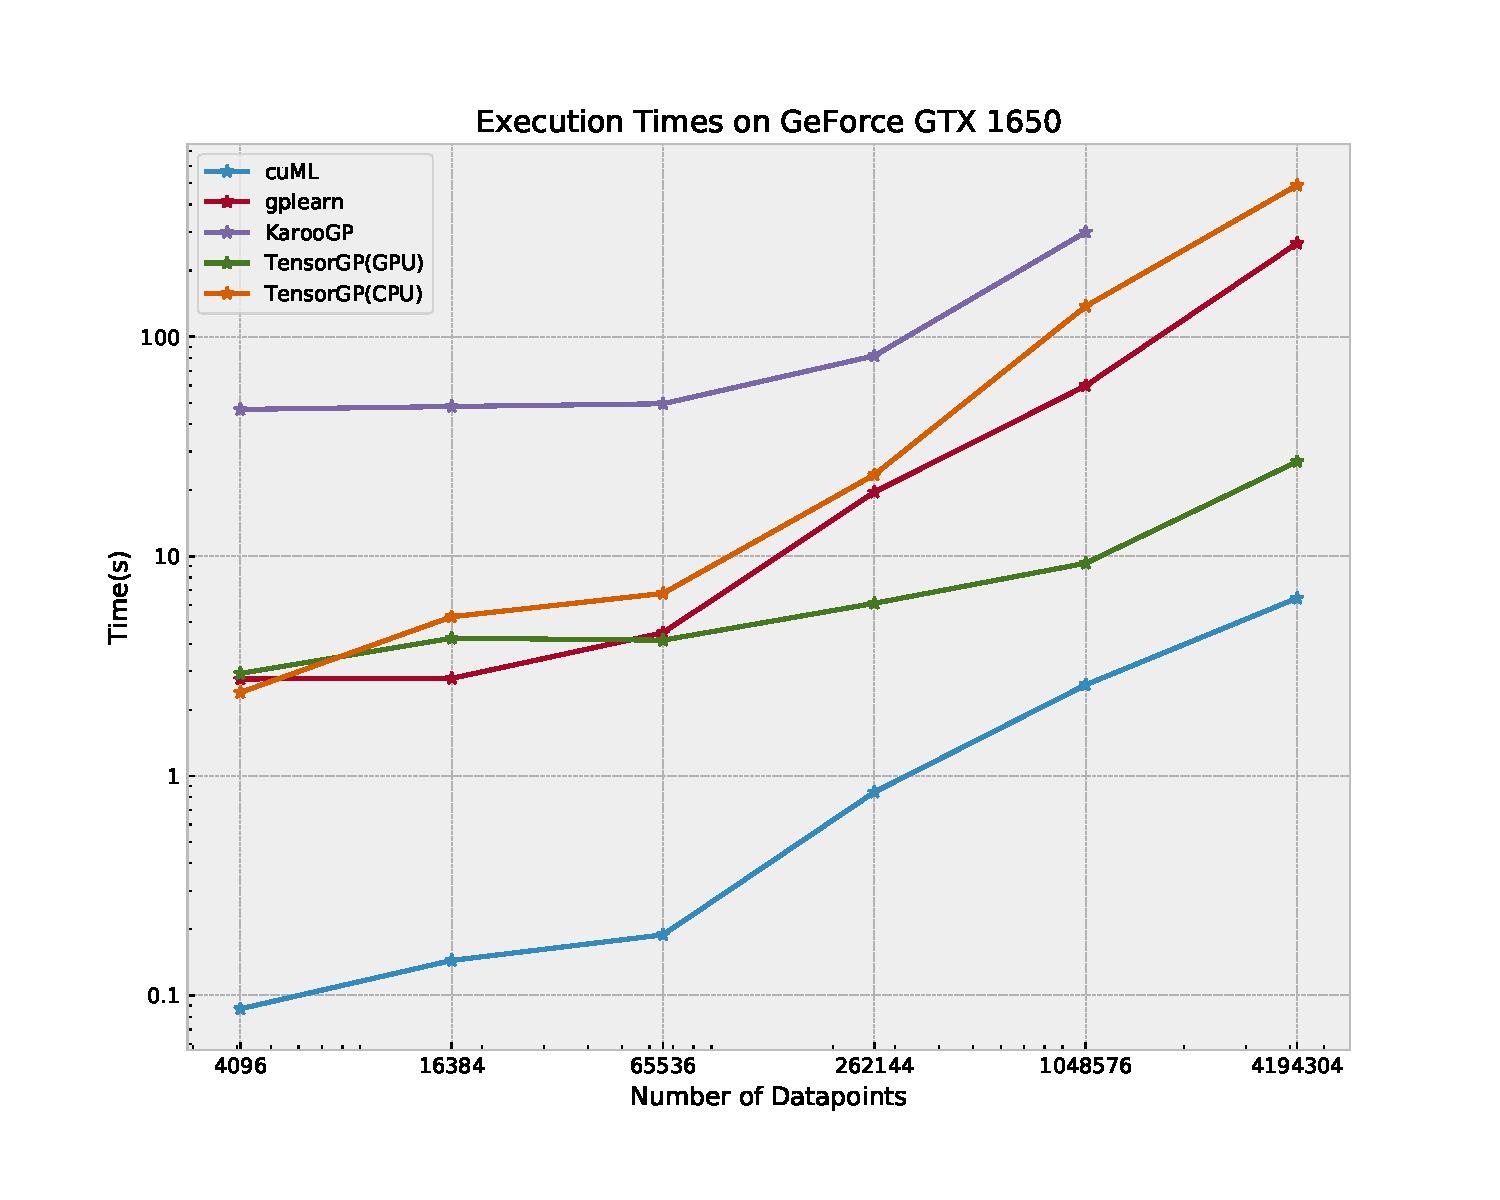
\includegraphics[scale=0.55]{images/ExecutionTimes.pdf}
  \caption{LogLog Plot of Execution Time for various libraries. The number of datapoints considered exponentially increases from $4096$ to $4$ million}
  \label{fig:exectimes}
\end{figure}

\begin{table}[htbp]
  \caption{Table containing mean and standard deviation of execution time across $10$ runs in milliseconds across different libraries. NaN denotes that the test took more than $2$ hours to complete}
  \begin{adjustbox}{width=\columnwidth,center}
    \begin{tabular}{llrrrrrr}
      \toprule
      \textbf{\# Rows} & {} &  4096 & 16384 & 65536 & 262144 & 1048576 & 4194304 \\
      \midrule
      \textbf{cuML} & mean &    86.92 &   144.35 &   188.84 &    843.21 &    2598.17 &    6447.31 \\
      & std &     0.60 &     6.27 &     8.34 &     11.49 &      18.51 &      25.29 \\
      \midrule
      \textbf{gplearn} & mean &  2761.76 &  2778.81 &  4484.50 &  19593.88 &   59786.29 &  266294.33 \\
      & std &   528.24 &   405.48 &   305.91 &    433.91 &     718.06 &    6096.38 \\
      \midrule
      \textbf{KarooGP} & mean & 46628.83 & 48079.62 & 49489.57 &  81830.44 &  299534.68 &        NaN \\
      & std &  8706.63 &  7253.72 &  7696.79 &  11818.43 &   11527.51 &        NaN \\
      \midrule
      \textbf{TensorGP(GPU)} & mean &  2926.20 &  4236.78 &  4147.59 &   6107.87 &    9298.63 &   26983.58 \\
      & std &   157.08 &    81.59 &    61.61 &    135.50 &     219.44 &     264.13 \\
      \midrule
      \textbf{TensorGP(CPU)} & mean &  2397.36 &  5303.11 &  6773.76 &  23515.70 &  137527.62 &  489625.81 \\
      & std &    72.89 &   115.62 &    38.57 &    223.69 &     414.81 &    2055.17 \\
      \bottomrule
      \end{tabular}      
    \label{tab:execavgs}
  \end{adjustbox}
\end{table}

From \cref*{tab:execavgs}, we note that cuML takes $6.4$ seconds on inputs of size $4$ million, wheras gplearn takes around $266.3$ seconds on the same input, after parallelization using $8$ jobs. When taking a mean average of runtime across all datasets and runs, we achieve an average speedup of $27$x in training time with respect to gplearn, with a maximum speedup of $41$x in the $4$ million row dataset.

Since KarooGP uses the TensorFlow \textit{graph} execution model, it is possible that more time is spent in building the execution DAG before evaluating it. In comparison, gplearn (which is already parallelized using $8$ jobs), uses numpy for fitness computations, which can exploit the AVX SIMD intructions on Intel CPUs to achieve greater parallelism. 

We believe that this job based parallelization again explains why gplearn is faster than TensorGP(CPU) - which is also optimized to utilize AVX SIMD instructions using TensorFlow's CPU backend.

From the graph in \cref*{fig:exectimes}, as well as \cref*{tab:execavgs}, we see that the TensorGP(GPU) approach consistently beats gplearn, KarooGP and TensorGP(CPU) on datasets with more than $65536$ points. Since TensorGP(GPU) uses TensorFlow's GPU backend with eager execution, time is not spent in building an optimized computation DAG for every program. This in turn increases the speed of parallel evaluation.

When comparing cuML to the rest of the libraries in \cref{fig:exectimes} and \cref{tab:execavgs}, we note that cuML is the fastest among all libraries on all inputs. We are faster than TensorGP(GPU) also, since cuML batches the computation of fitness across the entire population and dataset. 

\subsection{Variation of Fitness}
\label{subsec:fitnessvar}


For cuML, \cref{fig:besttrainfit} showcases the variation of the fitness score of the best tree in every generation for all datasets. 

\begin{figure}[htbp]
  \centering
  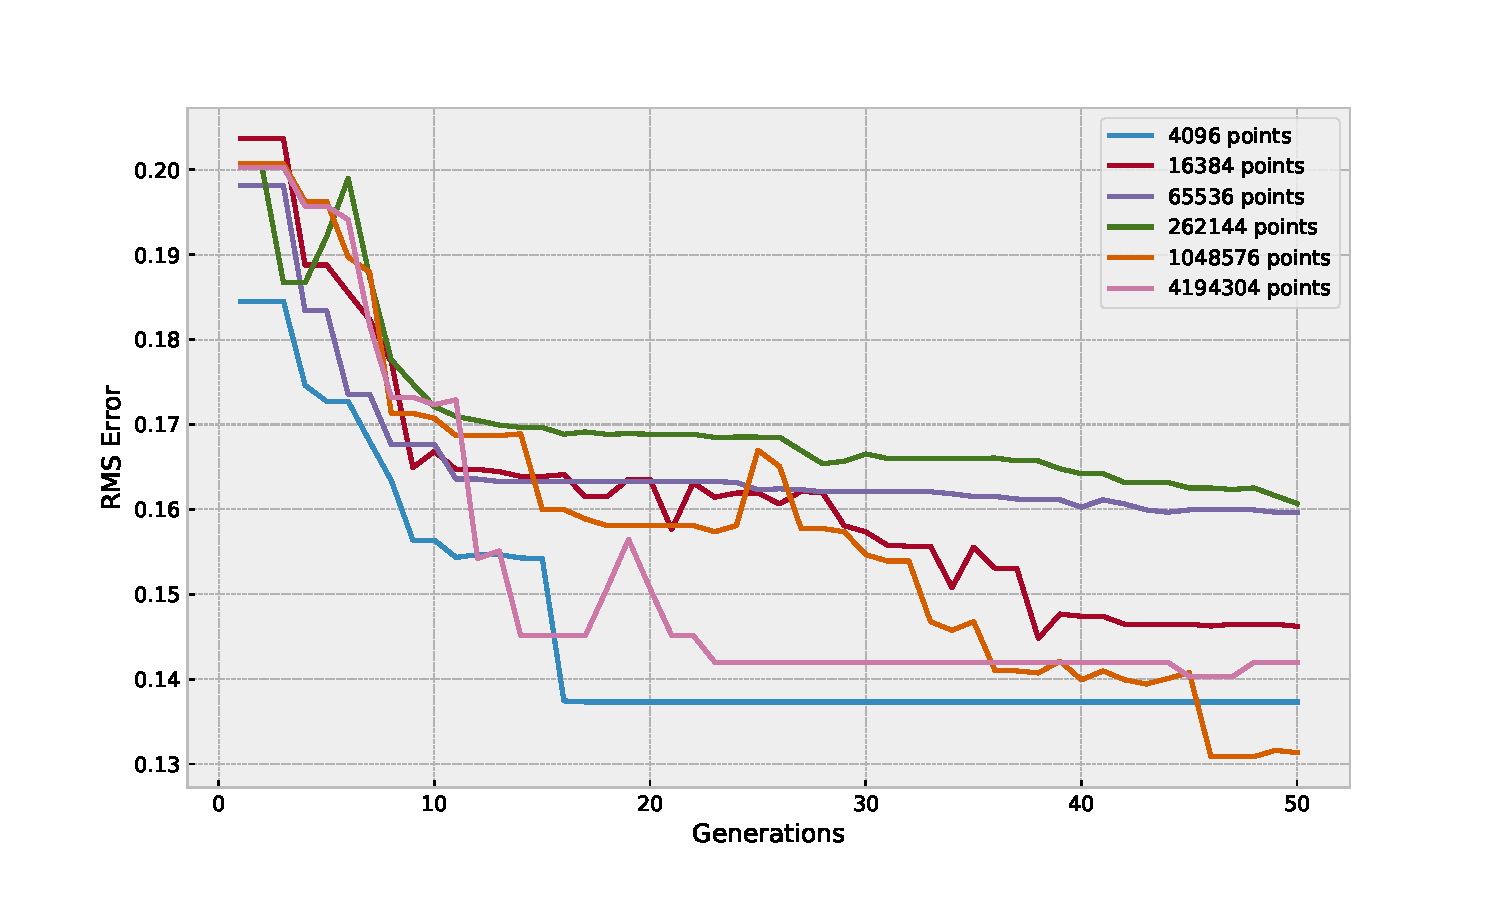
\includegraphics[scale=0.59]{images/RMSError.pdf}
  \caption{Plot showcasing the variation of Root Mean Square(RMS) error of with the number of generations. The error value corresponds to the fitness value of the optimal tree in every generation. }
  \label{fig:besttrainfit}
\end{figure}

It is easy to notice that the $1$ million row test set displays a monotonically decreasing error with increasing number of generations. However, we notice that the overall fitness value doesn't decrease even with an increase in the total number of evaluation datapoints in the same domain. Using this, we can conclude that bigger and more granular datasets do not help if we are performing symbolic regression to find the Pagie Polynomial, a result in line with \citep{baeta2021speed}.

We take the analysis a bit further and examine the variation of fitness values for both gplearn and cuML on the $1$ million row dataset, since both libraries implement the same types of mutations. \Cref{fig:gplearnvscuML1mil} visualizes this variation. We note that both cuML and gplearn exhibit similar behaviour with respect to non-increasing fitness values with increasing number of generations. 

\begin{figure}[h]
  \centering
  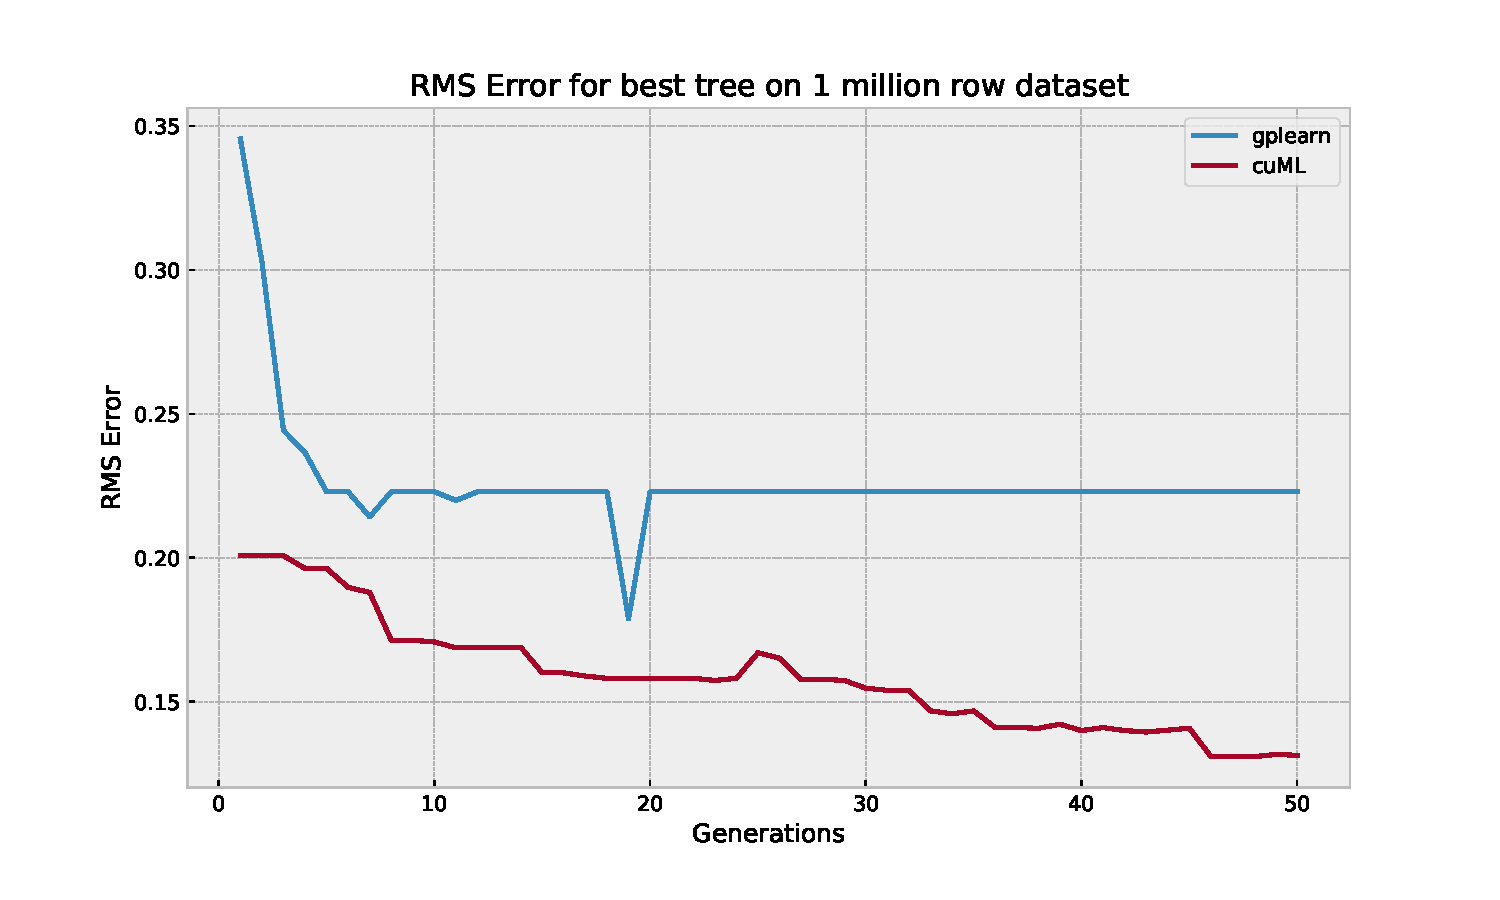
\includegraphics[scale=0.59]{images/RMSErrorGPLEARN.pdf}
  \caption{Plotting the variation of the best tree fitness(during training) with number of generations for both cuML and gplearn. The fitness values correspond of the $1$ million row dataset for both libraries.}
  \label{fig:gplearnvscuML1mil}
\end{figure}

We note that \cref{fig:gplearnvscuML1mil} \textbf{cannot} be used to determine which library produces better results for symbolic regression in general. This is because the final fitness value achieved is highly sensitive to the initialization of programs, which is randomized. Rather, the only goal of \cref*{fig:gplearnvscuML1mil} is to help us verify similar convergence behaviour of fitness values for both gplearn and cuML on the same datasets, when initialized with the same hyperparameters.

\subsection{Evaluation Effects}
\label{sec:evaleffects}
In this section, we inspect the effect of cuML's execution kernel with respect to the percentage of GPU Time consumed. To do this, we use the command-line GPU profiler \textbf{nvprof}, which gives us a runtime summary of CUDA kernels memory transfers. \Cref{tab:nvprofexec} summarizes the amount of time spent by the execute kernel with respect to all GPU activities. 

\begin{table}[htbp]
  \caption{Summarizing the time spent by the execution kernel as a summary of all GPU activities across $10$ runs. All results were collected using the command line tool \textbf{nvprof}}
  \begin{center}
    \begin{tabular}[c]{cc}
      \toprule
      \textbf{Number of Rows} & \textbf{Execution Time (\%)} \\
      \midrule
      4096    & 32.20\\
      16384   & 75.29\\
      65536   & 70.84\\
      262144  & 87.04\\ 
      1048576 & 86.15\\
      4194304 & 77.61\\
      \bottomrule
    \end{tabular}
    \label{tab:nvprofexec}
  \end{center}
\end{table}

The values in \cref*{tab:nvprofexec} indicate to us that the execution step is still the bottleneck in the run of the algorithm. Thus, on an average $71.52\%$ of GPU time is spent in the execution kernel.

In the next chapter, we shall list out some conclusions and possible optimizations and feature additions to the current implementation of cuML. 
